\chapter{PERCEPTION TACTILE}
Sens du toucher : (déf) système qui peut mesurer une propriété donnée d’un objet ou d’un phénomène, au travers d’un contact physique entre le système et l’objet. [Lederman SJ. Tactual Perception]\par
Le sens du toucher pour certains animaux est primordial. Les araignées sont très sensibles au toucher mais ne voient pas la lumière, l’obscurité et les formes basiques [Barth’2016…]. Les araignées apprennent plus sur leur environnement en ressentant les vibrations qu’en utilisant leurs yeux. Elles arrivent à faire la distinction en les différentes vibrations (insert dans la toile, vent qui souffle, autre araignées sur la toile, …).\par
Diap presentation\par
Le sens du toucher chez les mammifères et humains :\par
…Les Mammifères […]\par
…Le premier sens développé chez le fétu – au bout de 7 semaines, haptonomie - \par
Sens de nature complexe et non intuitive. Ce n’est pas une simple transduction d’une propriété physique en un signal électrique. Elle peut prendre plusieurs formes de la détection d’une texture, d’une forme, d’une blessure, d’un échange et autre. Les dernières avancées dans le domaine de l’haptique, des neurosciences cognitives et psychologiques.\par
Par rapport au sens de l’ouïe ou de la vue, le toucher reste encore une quantité définie. Dans les prochains paragraphes, un état de l’art sur la mécanique de la peau, les systèmes mécanorécepteurs de la peau jusqu’au système somatosensoriel va être établi à partir des dernières études faites en haptique.\par

\section{Procédure d’exploration}
Pour satisfaire ces besoins la peau doit être capable distingue et faire émerger différentes propriétés. Pour ce faire. La main interagi avec un objet/surface selon plusieurs méthodes. Ces méthodes recensé dans une étude de Lederman et Klatzy sont nommé « exploratory procedure » or EP for short (Lederman \& Klatzky 1987):\par
\begin{figure}[!h]
	\centering
	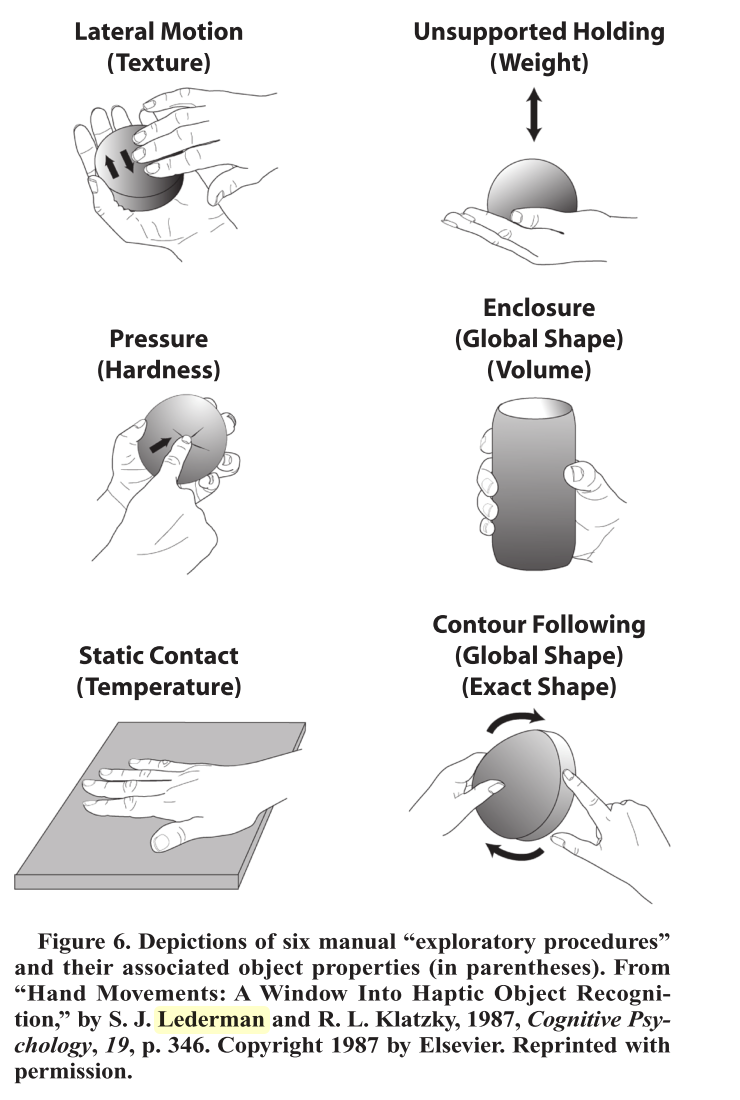
\includegraphics[width=7cm]{1_Bible/Photos/Psychology/proc_explo.png}
	\caption{Procédure d’exploration [] }\label{proc_explo}
\end{figure}

\section{Dimension du toucher}
Les EP, vu précédemment, servent notamment à renseigner sur la nature de l’objet/surface manipuler, qui sont caractérisé par les grandeurs physique et psychophysique suivante (Okamoto et al. 2013):
\begin{itemize}
	\item Texture;
	\begin{itemize}
		\item Rugueux/lisse;
		\begin{itemize}
			\item Macro-echelle (coarse);
			\item Micro -echelle (fine);
		\end{itemize}
		\item Dur/mou;
		\item Friction;
		\begin{itemize}
			\item Humide/sec;
			\item Glissant/collant;
		\end{itemize}
	\end{itemize}
	\item Température : Chaud/Froid;
	\item Forme : global/exact;
	\item Poids.
\end{itemize}
La texture regroupe plusieurs dimension et non seulement des information de rugosité. (voir liste au dessus).\par
Dualité de la perception de la rugosité : La rugosité d’une surface est perçu à deux échelles : Une macro-échelle, de l’ordre du millimetre et une micro-echelle de l’ordre du micrometre (voire nanometre). Cette difference d’échelle s’explique par les mecanisme du toucher qui encode la rugosité. La macro echelle vient du fait que les MR SA1 encode les informations de rugosité localement, là où peau et surface font contact. De ce fait, les limite de perceptions dépendent de l’acuité spatiale du sens du toucher. (threshold autour de 1mm). La micro-echelle dépend des MR PC qui encode les vibration créent par le doigt parcourant la surface. Ces vibrations se propagent dans tout le doigt, la paume des mains et vont même jusqu’au poignet. Des détails aussi fin que de qq centaine de nanomètre peuvent induire de telle vibration.\par
…Les parties les plus sensibles de notre corps humain sont les parties telles que : la figure, l’arrière de la nuque, les mains, le haut du bras, le torse, entre les jambes et la plante des pieds.\par
Et les changements d’état de celui-ci, glissement d’un objet, caresse,…\par
Le système somatosensoriel traite les données spatiotemporelles provenant des mécanorécepteurs [glissement, vibration], thermorécepteur [température] et nocicepteur [blessure] compris dans la peau.\par


\section{Taux de transfert d’information tactile}
...

\section{Types de toucher}
Outre tous les caractéristiques biologiques de la peau et les informations qu’il est possible d‘en retirer quant à son importance dans la sensation d’une surface/d’un objet (i.e.: la souplesse/dureté de la surface de contact, sa température, sa texture, sa forme, etc.), il est intéressant de noter que notre perception se découpent en différents types de toucher, aux caractéristique différentes (exemple : récepteur stimulé). En tout on peut distinguer jusque quatre type de toucher : de manipulation, d’exploration, communicatif et protectif.\par

\subsection{Toucher de manipulation}
Type de peau : glabre\par

Le toucher de manipulation est spécifique à la peau glabre est aussi celui qui a été le plus étudié.

\subsection{Toucher d’exploration}
Type de peau : Glabre ; et Poilu pour la navigation\par
Le toucher d’exploration est…

\subsection{Toucher communicatif}
Type de peau : Poilu\par
Le toucher communicatif est …

\subsection{Toucher protectif}
Type de peau : Poilu\par
Le toucher est …




